\documentclass[12pt,a4paper]{report} 

\usepackage[utf8]{inputenc}
\usepackage[T2A]{fontenc} 
\usepackage[russian]{babel}

\usepackage{cmap}
\usepackage{mathtools}
\usepackage{amssymb}
\usepackage{listings}
\usepackage{minted}

\usepackage[top=1in, bottom=1in, left=1in, right=1in]{geometry}
\usepackage{setspace}
\usepackage{indentfirst}

\usepackage{tocloft}

\setlength\parindent{24pt}
\lstset{language=Python}

\DeclarePairedDelimiter\floor{\lfloor}{\rfloor}

\newcommand*\mean[1]{\overline{#1}}
\newcommand\abs[1]{\left|#1\right|}

\setcounter{secnumdepth}{0}

\begin{document}

\begin{titlepage}

\center % Center everything on the page
 
%----------------------------------------------------------------------------------------
%	HEADING SECTIONS
%----------------------------------------------------------------------------------------

\textsc{\large Санкт-Петербургский Государственный}\\
\textsc{\large Политехнический Университет}\\
[9cm] 

%----------------------------------------------------------------------------------------
%	TITLE SECTION
%----------------------------------------------------------------------------------------

\begin{spacing}{2}
{ \huge \bfseries Распределенная реализация алгоритма поиска похожих объектов }\\[1.5cm]
\end{spacing}

%----------------------------------------------------------------------------------------
%	AUTHOR SECTION
%----------------------------------------------------------------------------------------

\begin{minipage}{0.4\textwidth}
\begin{flushleft} \large

\end{flushleft}
\end{minipage}
~
\begin{minipage}{0.4\textwidth}
\begin{flushright} \large
\emph{Выполнили:}\\
\textsc{Безруков Вадим}\\ 
\textsc{Панов Лев}\\ 
\textsc{Толмачев Александр}\\ 
\textsc{Шеина Екатерина}\\ 
\emph{гр. 63601/2}\\
[0.5cm] 
\emph{Преподователь:}\\
\textsc{Клавдиев Д.В.}\\ 
\end{flushright}
\end{minipage}\\

%----------------------------------------------------------------------------------------
%	DATE SECTION
%----------------------------------------------------------------------------------------

\vfill % Fill with whitespace

{\large Санкт-Петербург, 2014}

\end{titlepage}

\tableofcontents

\newpage

\section{Постановка задачи}

Имеется большой объем данных, содержащих информацию о посещении пользователями интернет-сайтов. Данные представляют собой текстовые файлы, каждая строчка которых содержит информацию о посещении определенным пользователем определенного сайта. Пользователи и сайты определяются своими уникальными идентификаторами.

Требуется реализовать алгоритм, который по имеющемуся массиву данных и номеру конкретного сайта определяет тех пользователей, которые не посещали данный сайт, но с высокой вероятностью им заинтересуются. Реализация алгоритма должна быть распределенной, то есть должна позволять обрабатывать данные на кластере из нескольких машин. Также требуется провести испытания полученного решения и исследовать зависимость времени, затрачиваемого на получение результата, в зависимости от количества используемых вычислительных ресурсов.

\section{Описание метода решения}

Идея подхода, выбранного нами для решения задачи, состоит в следующем. 
Каждый пользователь посещает какие-то сайты чаще, какие-то реже. Можно предположить, что чем чаще пользователь посещает сайт, тем более этот сайт ему интересен. Таким образом, можно составить картину интересов пользователя, основываясь на частоте посещений (посчитать для данного пользователя рейтинги посещаемых им сайтов).
В свою очередь, каждый сайт можно охарактеризовать тем, какие пользователи и насколько часто его посещают. Разумно предположить, что похожие сайты посещают похожие пользователи (имеющие общие интересы). Соответственно, можно определить, насколько два сайта похожи, по тому, насколько похожи их аудитории. Далее, имея информацию о том, какие сайты в какой мере интересны для пользователя, и о том, насколько сайты похожи между собой, можно предсказать, насколько пользователю будет интересен некоторый сайт, на котором он не был: можно оценить рейтинг для данного сайта, используя известные рейтинги посещаемых им сайтов с учетом того, насколько каждый из посещаемых сайтов похож на данный.

Таким образом, для решения задачи требуется выполнить следующие этапы:
\begin{enumerate}
\setlength\itemsep{0em}
\item Вычислить рейтинги сайтов для каждого пользователя.
\item Определить, насколько сайт, поданный на алгоритму вход, похож со всеми остальными сайтами.
\item Предсказать рейтинг данного сайта для всех пользователей, которые его не посещали.
\end{enumerate}
Затем остается отсортировать пользователей по убыванию предсказанного рейтинга и выдать заданное число пользователей из начала этого списка.

\subsection{Вычисление рейтингов} 

Исходные данные содержат информацию о том, какие сайты каждый конкретный пользователь сколько раз посещал. Располагая такой информацией, можно вычислить пользовательский рейтинг для сайта следующим образом:
\begin{equation}
r_{u,s} = \frac{num\_visits_{u,s}}{  \max\limits_{s \in Visited(u)} num\_visits_{u,s}} ,
\end{equation}
где $num\_visits_{u,s}$ -- число посещений сайта $s$ пользователем $u$, $Visited(u)$ -- множество сайтов, посещенных пользователем $u$. Таким образом, рейтинг представляет собой число из интервала $[0,1]$ и отражает то, какой популярностью данный сайт пользуется у данного пользователя.

\subsection{Определение похожести сайтов} 

Каждый из рассматриваемых сайтов можно охарактеризовать тем, насколько он популярен у тех или иных пользователей, то есть вектором пользовательских рейтингов, вычисленных на предыдущем этапе. Тогда, введя меру похожести для этих векторов, можно определить то, насколько два сайта похожи между собой. В качестве такой меры похожести мы используем коэффициент корреляции Пирсона: 
\begin{equation}
corr_{s_1, s_2} = \frac{ \sum\limits_{u \in Visited(s_1, s_2)} (r_{u,s_1} -  \mean{r}_{s_1}) (r_{u,s_2} -  \mean{r}_{s_2}) }
{ \sqrt{ \sum\limits_{u \in Visited(s_1, s_2)} (r_{u,s_1} -  \mean{r}_{s_1})^2 } \sqrt { \sum\limits_{u \in Visited(s_1, s_2)} (r_{u,s_2} -  \mean{r}_{s_2})^2 } },
\end{equation}
где $Visited(s_1, s_2)$ -- множество пользователей, посетивших оба сайта $s_1$ и $s_2$, $r_{u,s}$ -- рейтинг сайта $s$ для пользователя $u$, $\mean{r}_{s}$ -- средний рейтинг сайта $s$ по всем пользователям.

\subsection{Предсказание рейтингов} 

Пусть $t$ -- сайт, поданный на вход алгоритму. Тогда для каждого из пользователей, которые не посещали этот сайт, можно оценить рейтинг следующим образом:
\begin{equation}
\widetilde{r}_{u,t} = \mean{r}_u + \frac{\sum\limits_{s \in Visited(u)}{ (r_{u,s} - \mean{r}_u) \, corr_{s,t}} }{ \sum\limits_{s \in Visited(u)}{\abs{corr_{s,t}}} } ,
\end{equation}
где $\mean{r}_u$ -- средний рейтинг посещаемых сайтов для пользователя $u$, $Visited(u)$ -- множество сайтов, посещаемых пользователем $u$. То есть предсказываемый рейтинг вычисляется как сумма среднего рейтинга по посещаемым сайтам и средневзвешенного отклонения от среднего, где веса -- коэффициенты корреляции для посещаемого сайта и сайта, для которого предсказывается рейтинг.

\newpage

\section{Описание технологии Apache Spark}

Для реализации алгоритма мы выбрали технологию распределенных вычислений Apache Spark. Это относительно новый фреймворк для анализа больших массивов данных, уже получивший довольно большую популярность. Разработчики Spark заявляют о его высокой производительности по сравнению с Apache Hadoop, вплоть до 100-кратного превосходства для некоторых задач. 

Apache Spark является проектом с открытым исходным кодом. Работа над этим фреймворком начиналась в 2009 году в рамках научно-исследовательского проекта в Калифорнийском университете Беркли. В 2013 году проект перешел в Apache Software Foundation. А в 2014 году он стал одним наиболее приоритетных проектов Apache.

\subsection{Resilient Distributed Datasets} 

В основе фреймворка лежит концепция RDD (Resilient Distributed Dataset) -- абстракция для высокоэффективной и отказоустойчивой работы с распределенными массивами данных. RDD -- это неизменяемая коллекция объектов, распределенная по машинам кластера. Они может постоянно находятся в оперативной памяти, что позволяет обеспечивать высокую скорость доступа к данным при вычислениях. Например, при RDD размером до 39 ГБ гарантируется скорость доступа менее 1 с. 

С точки зрения интерфейса RDD представляет собой единую коллекцию данных. Spark сам заботится о ее разбиении на части и размещении в оперативной памяти и на жестких дисках машин, а также о связи частей между собой. В то время как пользователь работает с RDD как с локальной коллекцией данных. 

Вычисления в Apache Spark организуются как последовательности преобразований над RDD. История преобразований коллекции данных сохраняется, поэтому в случае сбоев утраченная часть коллекции может быть заново восстановлена. Это обеспечивает устойчивость к сбоям (fault-tolerance). Также вычисления происходят ``ленивым'' образом: непосредственно преобразования данных происходят только тогда, когда требуются результаты вычислений. Это позволяет организовывать вычисления более оптимально -- группировать определенные преобразования и выполнять их партиями, более эффективно распараллеливать независимые преобразования, а также вообще не выполнять тех вычислений которые не требуются для получения конечного результата.

\subsection{Способы хранения данных} 

Если объем данных таков, что они не помещаются в оперативную память машин кластера, Spark будет выгружать их на жесткий диск. При это есть возможность указать, какие данные где могут располагаться -- в оперативной памяти (для данных, к которым требуется частое обращение), в оперативной памяти и на жестком диске, только на жестком диске, какие данные сохранять в сериализованном виде, какие нет и т.д. Spark предоставляет пользователям гибкую настройку в вопросе использования памяти, которая позволяет оптимально использовать имеющиеся ресурсы.

Возможность хранения данных в оперативной памяти предоставляет большие преимущества для ряда вычислительных задач и является одной из сильных сторон фреймворка Spark. Для сравнения, Аpache Hadoop не имеет такой возможности и записывает промежуточные результаты map-reduce операций на жесткие диски машин, что очень затратно и существенно снижает производительность. Поэтому для задач, которые требуют значительного использования промежуточных данных, Spark работает до ста раз быстрее, чем Apache Hadoop. 

Загружать исходные данные Spark позволяет как с локальной файловой системы машин, так и из распределенных файловых систем и хранилищ: HDFS, Amazon S3, Cassandra, HBase и т.д. 

\subsection{Интерфейсы взаимодействия} 

Spark предоставляет API для написания программ на Java, Python и Scala. Наиболее поддерживаемым языком является Scala, т.к. Spark сам написан на Scala и все основные тесты написаны на Scala. Благодаря функциональной выразительности предоставляемого API программы для Apache Spark получаются короче и проще, чем для Apache Hadoop.

Работа с RDD происходит при помощи вызова методов, предоставляемых в API. Методы делятся на две группы: Transformations и Actions. Методы, относящиеся к группе Transformations, производят преобразование коллекции данных и возвращают новую RDD (например, методы \texttt{map} и \texttt{reduceByKey}). Методы, относящиеся к Actions, выполняют операции с коллекцией данных и возвращают конечный результат (например, метод \texttt{count}, вычисляющий количество элементов в коллекции, или метод \texttt{count} который позволяет сохранить коллекцию данных на локальный диск). Все методы из Transformations ленивые, то есть их выполнение откладывается до вызова первого метода из Actions.

\subsection{Архитектура распределенных вычислений} 

Приложения для Spark выполняются на кластере как самостоятельные наборы процессов, управляемые объектом SparkContext в основной программе (driver program). SparkContext подключается к менеджеру кластера (cluster manager), который отвечает за управление вычислениями. После подключения Spark запускает исполнителей (executor) на узлах кластера -- процессы, которые выполняют вычисления и отвечающими за хранение данных на конкретном узле. После этого Spark загружает программный код (упакованный в JAR архив или Python файлы) и рассылает задачи (task) по исполнителям.
\begin{figure}[h]
  \centering
  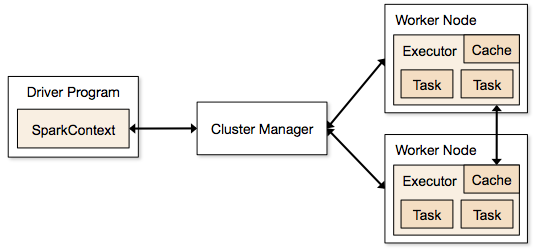
\includegraphics[width=0.65\textwidth]{cluster-overview.png}
  \caption{Схема архитектуры вычислений на кластере}
  \label{cluster-overview}
\end{figure}

\noindent Некоторые особенности такой архитектуры:
\begin{enumerate}
\setlength\itemsep{0em}
\item Каждое приложение получает свои процессы исполнителей, которые работаю пока запущено приложение и выполняют задачи в разных потоках. Таким образом приложения изолированы друг от друга, как со стороны планирования (каждый драйвер распределяет только свои задачи), так и со стороны исполнения (задачи из разных приложений выполняются на разных Java-машинах). Однако, это означает, что данные не могут разделяться между различными Spark приложениями без использования внешнего хранилища. 
\item Архитектура вычислений не зависит от используемого менеджера кластера. 
\item Поскольку драйвер распределяет задачи на кластере, он должен работать близко к рабочим узлам, предпочтительно в одной и той же локальной сети. 
\end{enumerate}
На данный момент Spark поддерживает три кластерных менеджера: 
\begin{itemize}
\setlength\itemsep{0em}
\item Standalone – простой менеджер кластера, поставляемый вместе со Spark. Позволяет быстро настроить кластер.
\item Apache Mesos – стандартный менеджер кластера, также позволяющий использовать Hadoop MapReduce и сервисные приложения.
\item Hadoop YARN – менеджер ресурсов в Hadoop 2.
\end{itemize}

\subsection{Рекомендации к оборудованию} 

\subsubsection{Системы хранения данных} 

Поскольку большинство встречаемых задач основываются на чтении входных данных с внешних системах хранения информации(в том числе Hadoop File System, или HBase) особенно важно разместить данные как можно ближе к системе. Рекомендуется следующее:
\begin{itemize}
\setlength\itemsep{0em}
\item По возможности, запускать Spark на идентичном железе с файловой системой HDFS. Проще всего настроить Spark в режиме standalone кластера на схожих узлах.  Также можно запускать Spark и Hadoop в общей кластерной группе с помощью систем для планирования заданий и управления кластерами типа MESOS,  Hadoop YARN.
\item Если нет возможности использования схожих узлов, то рекомендуется разместить узлы в локальной сети с HDFS(распределенной файловой системой).
\item На узлах, занимающихся вычислениями лучше не хранить “ленивые” данные типа HBase. (Правильнее разделять узлы для ленивых данных и для вычислительных узлов)
\end{itemize}

\subsubsection{Локальные диски}

Во время работы Spark используемые данные для вычислений хранятся в оперативной памяти, в то же время используются и локальные хранилища для данных не поместившихся в RAM. Рекомендовано использовать 4-8 дисковых хранилищ на узел настроенных без RAID. 

\subsubsection{Память} 

Spark может использовать  8Gb и до сотен гигабайт оперативной памяти на одной машине. Рекомендуется использовать не более 75\% от общего количества оперативной памяти на машине. Сколько именно оперативной памяти может потребоваться, напрямую зависит от поставленной задачи.  Эффективность использования памяти зависит и от эффективности жестких дисков и их файловой системы.

Также виртуальная машина Java не всегда ведет себя корректно с более чем 200 Gb оперативной памяти. Если имеются  машины с б\'{о}льшим колчеством оперативной памяти, можно использовать несколько виртуальных машин на одном узле.

\subsubsection{Сеть} 

В процессе работы Spark, множество распределенных данных передаются по сети. Использование 10-гигабитной или более быстрой сети -- лучший способ ускорить эту передачу. Это особенно важно для “распределенных вычислений” таких как group-bys, reduce-bys и SQL joins. Вы можете следить за передаваемыми данными Spark с помощью сетевого мониторинга.

\subsubsection{Многоядерные процессоры} 

Spark поддерживает многоядерные процессоры, т.к. создает минимальное разделение задач между потоками. Для сложных вычислений можно использовать 8-16 ядерные процессоры для ускорения обработки данных.

\section{Реализация алгоритма}

Мы реализовали алгоритм на языке Python, используя Python API фреймворка Apache Spark. Код программы приведен в приложении.

\section{Результаты испытаний}

TBD

\newpage


\newgeometry{top=0.75in, bottom=0.75in, left=0.5in, right=0.5in}

\section{Приложение. Исходный код программы.}

\inputminted[fontsize=\footnotesize]{python}{../look_alike.py}

\end{document}